\pdfminorversion=3
\documentclass[tikz]{standalone}
\usepackage{vuiprepstandalone}
\usepackage{alain2}
\usepackage[locale=FR]{siunitx}
\def\pathfig{02PerformancesSLCI/ex_Telechirurgie2/images}

\usetikzlibrary{shapes.geometric}
\usetikzlibrary{shapes.symbols}
\usetikzlibrary{shapes.arrows}

\begin{document}
\begin{tikzpicture}

\begin{scope}
\node[draw,rectangle, text width=4cm,align=center,fill=cyan!50] (a) {"requirement" \\Déplacement de l'outil};
\node[draw,rectangle, text width=4cm,align=left,text badly ragged,anchor=north,fill=cyan!50] (b) at (a.south) {id = "1" \\ Text = "positionner l'outil en minimisant l'effet d'une perturbation périodique."};
\end{scope}

\begin{scope}[yshift=-8cm,xshift=.5cm]
\node[anchor=south] (a1) {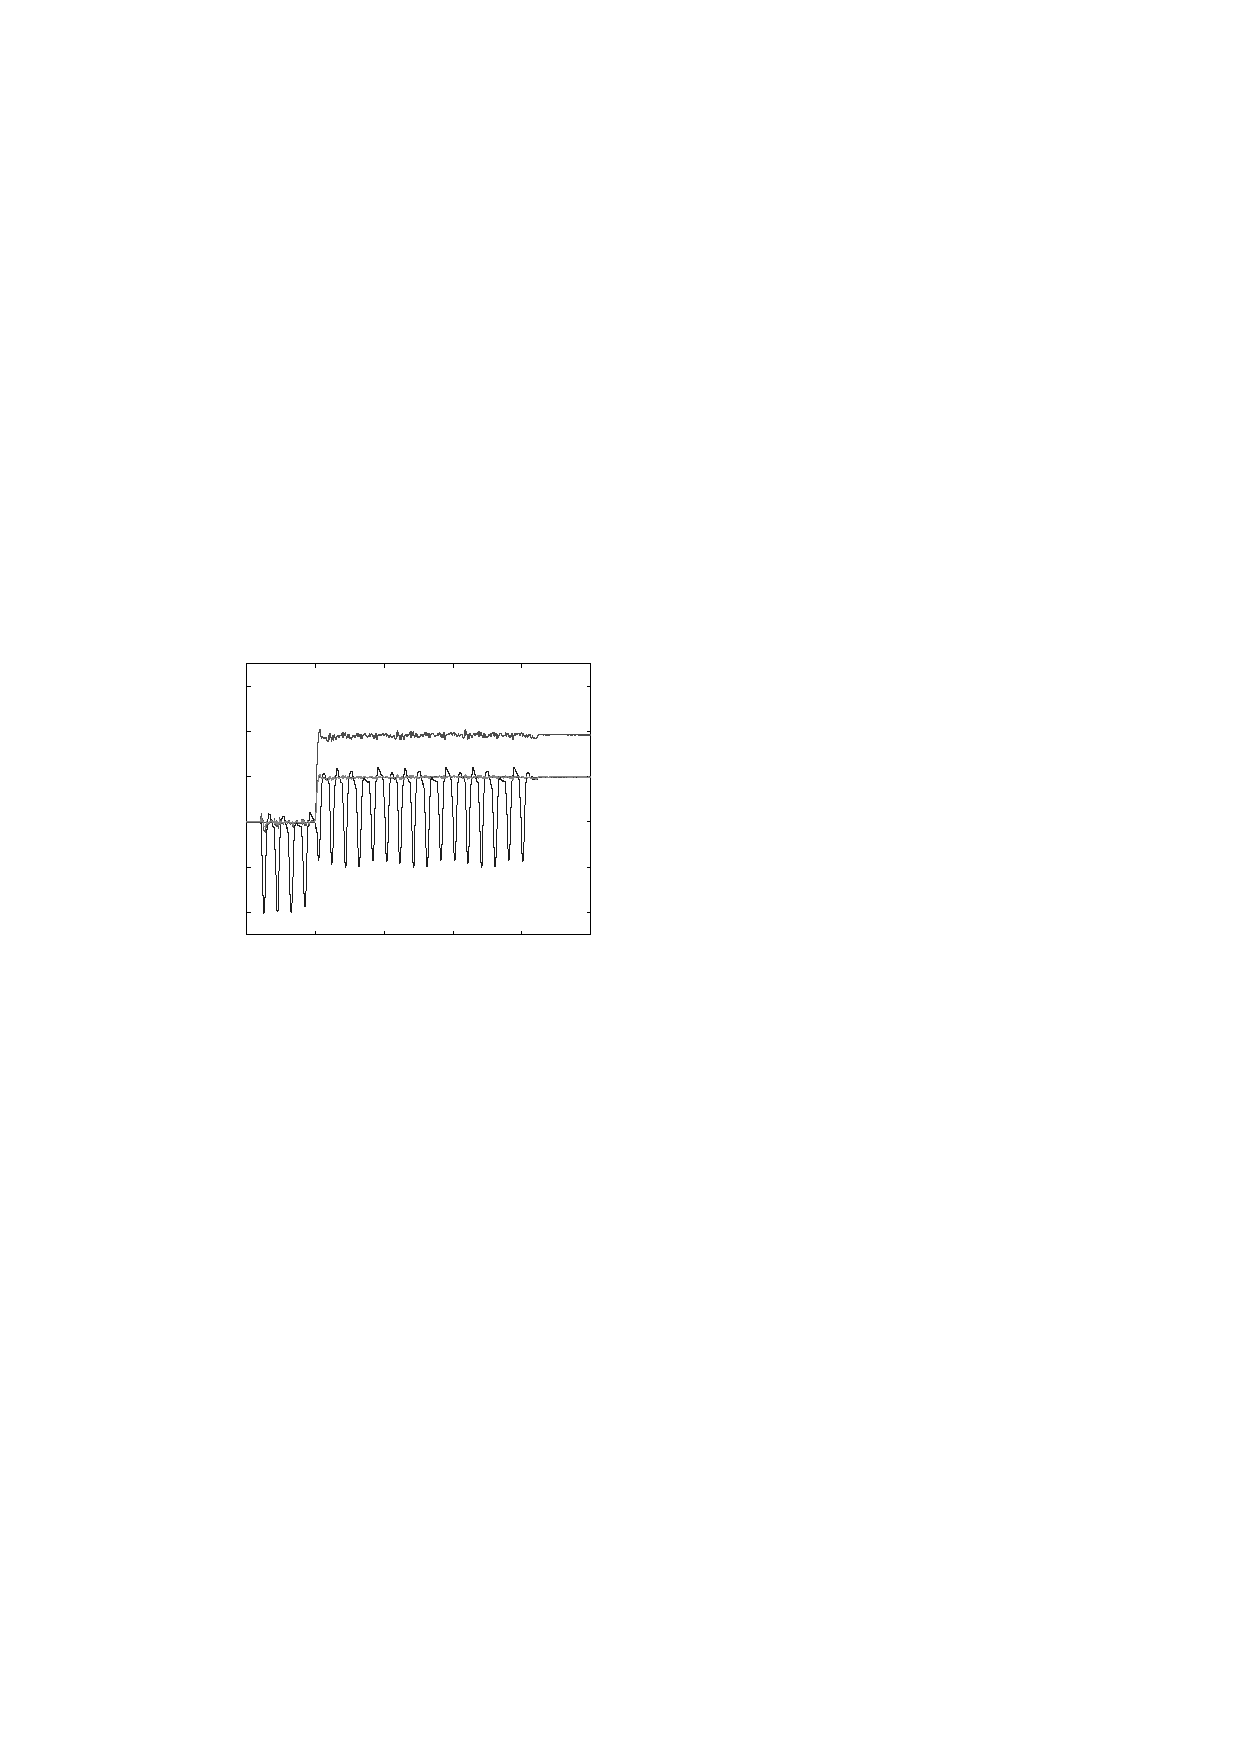
\includegraphics[width=6cm]{\pathfig/bilan_experience}};
\foreach \x/\t in {-3/0,-1.8/5,-.6/10,.6/15,1.8/20,3/25} \node[below] at (\x,0) {\t};
\foreach \y/\t in {0/-.02,.8/-.01,1.6/0,2.4/.01,3.2/.02,4/.03} \node[left] at (-3,\y+.5) {\num{\t}};
\node at (0,-.7) {Temps (s)};
\node[rotate=90] at (-4.2,2.5) {Position (en m) et force/100 (en N)};
\node[text width=6.5cm] at (-.5,-1.5) {Performances mesurées : au bout de 5 s, le maître impose un déplacement de 1 cm.};
\node at (0,5.1) {1 Hz};
\node[left] at (3,3.8) {Force};
\node[left] at (3,3.1) {Position maître};
\node[left] at (2,1.2) {Position esclave};
\end{scope}

\begin{scope}[yshift=-15.5cm,xshift=.5cm]
\node[anchor=south] (a1) {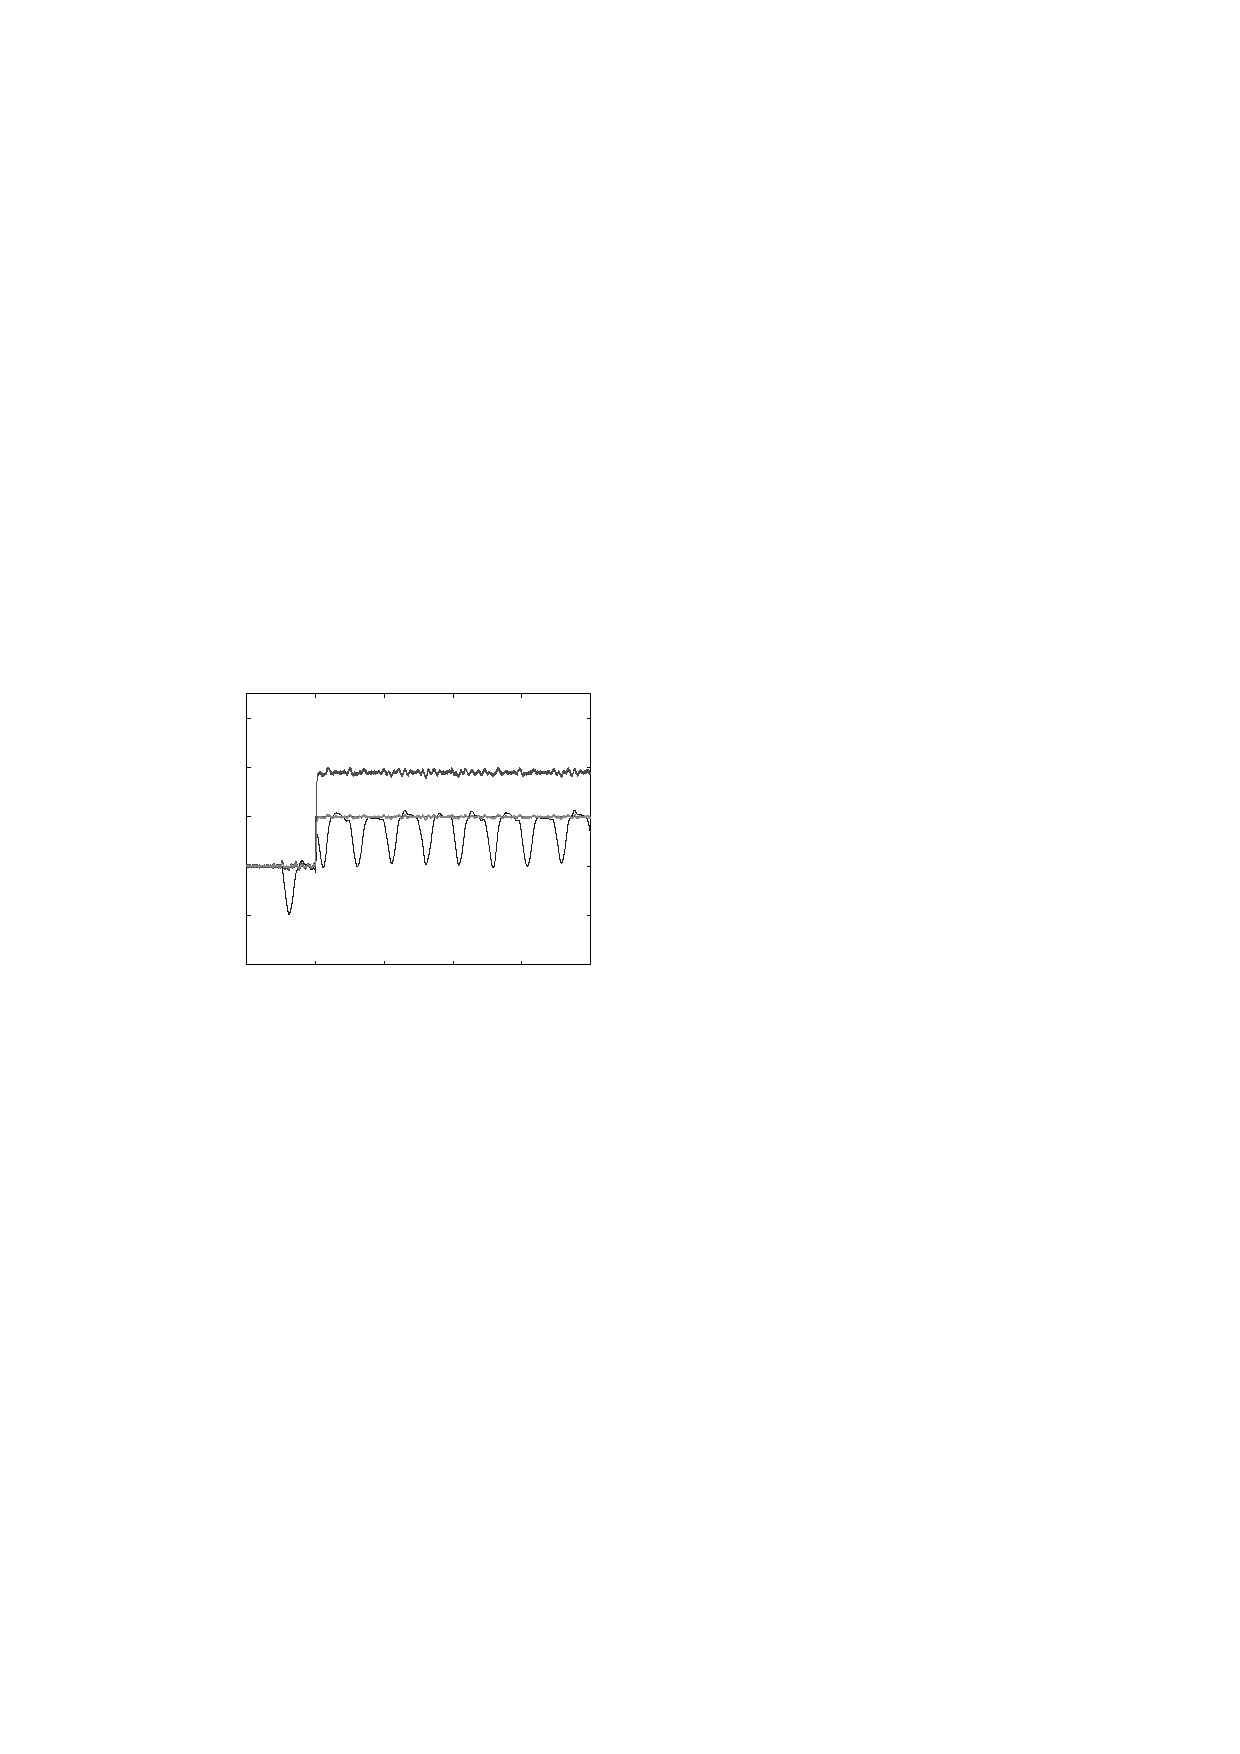
\includegraphics[width=6cm]{\pathfig/bilan_simulation}};
\foreach \x/\t in {-3/0,-1.8/2,-.6/4,.6/6,1.8/8,3/10} \node[below] at (\x,0) {\t};
\foreach \y/\t in {.1/-.02,.96/-.01,1.82/0,2.68/.01,3.54/.02,4.4/.03} \node[left] at (-3,\y) {\num{\t}};
\node at (0,-.7) {Temps (s)};
\node[rotate=90] at (-4.2,2.5) {Position (en m) et force/100 (en N)};
\node[text width=6.5cm] at (-.5,-1.5) {Performances mesurées : au bout de 2 s, le maître impose un déplacement de 1 cm.};
\node at (0,5.1) {1 Hz};
\node[left] at (3,3.7) {Force};
\node[left] at (3,2.9) {Position maître};
\node[left] at (2,1.6) {Position esclave};
\end{scope}


\node [single arrow, draw,minimum height=4.2cm,fill=cyan!30!gray!10] at (-6.5,-1) {Domaine du client};
\node [single arrow, draw,minimum height=4.2cm,fill=cyan!30!gray!10] at (-6.5,-5.5) {Domaine du laboratoire};
\node [single arrow, draw,minimum height=4.2cm,fill=cyan!30!gray!10] at (-6.5,-13) {Domaine de la simulation};

\node [double arrow, draw,rotate=90,minimum height=2.4cm,fill=cyan!30!gray!10] at (-10.25,-3.25) {écart};
\node [double arrow, draw,rotate=90,minimum height=5.4cm,fill=cyan!30!gray!10] at (-10.25,-9.25) {écart};
\node [double arrow, draw,rotate=90,minimum height=9.9cm,fill=cyan!30!gray!10] at (-12,-7) {écart};


\node[draw,rectangle,align=center,fill=cyan!50,minimum width=2.5cm,minimum height=1.5cm,left] at (-9,-1) {Système\\ souhaité};\
\node[draw,rectangle,align=center,fill=cyan!50,minimum width=2.5cm,minimum height=1.5cm,left] at (-9,-5.5) {Système\\ réel};
\node[draw,rectangle,align=center,fill=cyan!50,minimum width=2.5cm,minimum height=1.5cm,left] at (-9,-13) {Système\\ simulé};
\end{tikzpicture}
\end{document}